\subsection{Formación de imágenes}

Las \textbf{imágenes} se forman ya sea por \hl{reflexión} o \hl{refracción}, y es posible diseñar espejos y lentes que formen imágenes reales o virtuales.

\subsubsection{Introducción a los espejos}

\begin{wrapfigure}{r}{0.3\textwidth}
  \centering
  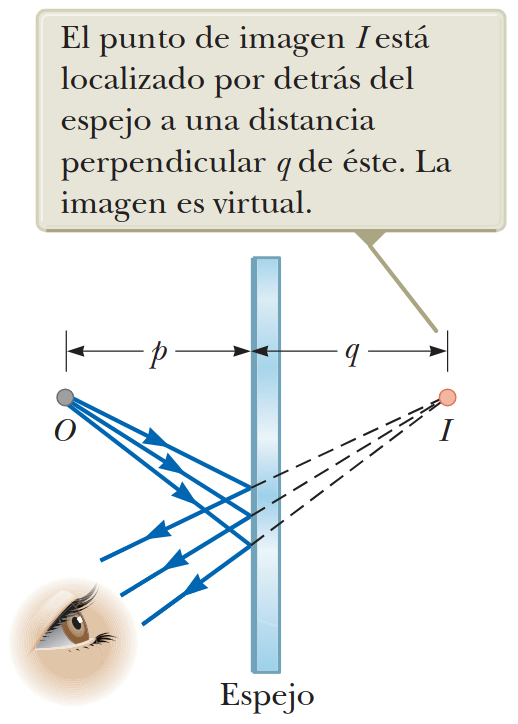
\includegraphics[width=\linewidth]{mirror.png}
  \caption{Imagen formada por reflexión en un espejo plano.}
  \label{fig:mirror}
\end{wrapfigure}
Los espejos forman imágenes a partir de la \textbf{reflexión} de la luz. Para entender cómo se forman las imágenes en un espejo, es importante entender los conceptos de reflexión y ángulos de incidencia y reflexión del haz de luz (ver sección \ref{sec:reflection}).

Cuando un rayo de luz incide sobre la superficie reflectante de un espejo, se refleja y puede llegar al ojo del observador. La \textbf{imagen} se forma en el punto donde los rayos reflejados (o sus prolongaciones) se interceptan.

\paragraph{Espejo plano}

Empecemos con la consideración del espejo más simple posible, el espejo plano. Imagine una fuente puntual de luz colocada en \(O\) en la figura \ref{fig:mirror}, a una distancia \(p\) de la superficie del espejo plano. La distancia \(p\) se llama \textbf{distancia objeto}. Los rayos luminosos \textit{divergentes}\footnote{Los rayos luminosos divergentes son aquellos que se alejan entre sí.} son reflejados por el espejo. Después de reflejarse, siguen un proceso de divergencia. Las líneas discontinuas de la figura \ref{fig:mirror} son extensiones de los rayos divergentes hacia atrás, hasta un punto \(I\), que se llama \textbf{imagen} del objeto \(O\). A la distancia \(q\) se la llama \textbf{distancia imagen}. 

Las imágenes están localizadas ya sea en un punto a partir del cual los rayos luminosos \textit{realmente} divergen, o en un punto a partir del cual los rayos luminosos \textit{aparentemente} divergen.

\begin{tcolorbox}[myconclusion]
    Independientemente del sistema de estudio, siempre se localizará las imágenes extendiendo hacia atrás los rayos divergentes, hasta el punto en que hacen intersección.
\end{tcolorbox}


\subsubsection{Imágenes reales y virtuales}

Las imágenes pueden clasificarse según varias características, una de ellas es si son \textit{reales} o \textit{virtuales}. Una imagen real es la que se forma cuando los rayos luminosos pasan por el punto de la imagen. Por otro lado, una imagen virtual es la que se forma cuando los rayos luminosos no pasan por el punto de la imagen, sino que parecen divergir desde el punto de la imagen. La imagen formada por el espejo de la figura \ref{fig:mirror} es virtual y está detrás del espejo.

La imagen vista de un objeto en un espejo plano \textit{siempre} es virtual. Más adelante veremos un ejemplo de imagen real.

\subsubsection{Aumento Lateral de una imagen}

\begin{wrapfigure}{r}{0.3\textwidth}
  \centering
  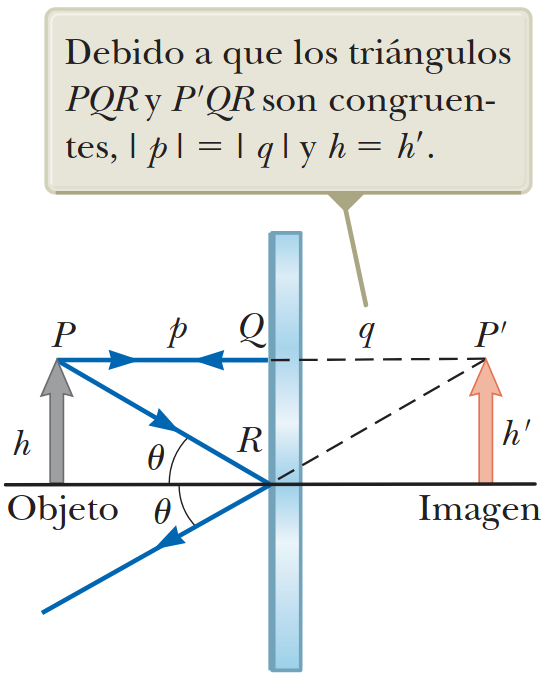
\includegraphics[width=\linewidth]{mirror_geometry.png}
  \caption{Construcción geométrica utilizada para localizar la \textbf{imagen} de un objeto en un espejo plano.}
  \label{fig:mirror_geometry}
\end{wrapfigure}
Veamos la figura \ref{fig:mirror_geometry}. Para poder determinar dónde se formará la imagen del objeto es necesario elegir dos rayos emitidos por el objeto. 

En este caso el objeto es una flecha. El punto \(P\) es el extremo superior de la flecha a una altura \(h\) sobre el eje horizontal. El primer rayo que vamos a elegir es el rayo que sale de \(P\), y va hasta \(Q\) que se refleja en el espejo plano sobre sí mismo. El segundo rayo que vamos a elegir es el rayo que sale de \(P\), y va hasta \(R\) que se refleja con un ángulo \(\theta\) con respecto al eje horizontal. 

Un observador que recibe el rayo \(PR\) reflejado, es capaz de ver la imagen virtual del objeto, que sería la flecha roja\footnote{Es importante entender que el objeto que se refleja es una flecha, los colores son únicamente para identificar la flecha original y la flecha reflejada}. Entonces, podría extender el rayo reflejado hasta la imagen virtual \(P'\), que está ubicada a una altura \(h'\) detrás del espejo sobre el eje horizontal.

Ya que los triángulos \(PQR\) y \(P'QR\) son congruentes, \(PQ=P'Q\). Por lo tanto, la imagen formada por un objeto colocado en frente a un espejo plano está tan lejos detrás del espejo como está el objeto delante del espejo. También \(h=h'\), por lo que la imagen virtual es del mismo tamaño que el objeto.

El \textbf{aumento lateral} \(M\) de una imagen se define como:
\begin{equation}
M = \frac{\text{altura de la imagen}}{\text{altura del objeto}} = \frac{h'}{h}
\label{eq:aumento_lateral}
\end{equation}
Esta definición general del aumento lateral para una imagen a partir de cualquier tipo de espejo también es válida para imágenes formadas por lentes.

Para cualquier espejo plano \(M=+1\), ya que la altura de la imagen es igual a la altura del objeto. El valor positivo de la amplificación significa que la imagen es vertical.

\subsubsection{Inversión aparente de un espejo plano}

La creencia de que un espejo plano ``invierte de derecha a izquierda'' es una ilusión perceptiva. En realidad, un espejo plano no invierte lateralmente (ni derecha-izquierda ni arriba-abajo); lo que invierte es la profundidad, es decir, el eje frente-detrás (o eje \(z\) en un sistema cartesiano tridimensional).

Cuando te colocas frente a un espejo plano, cada punto de tu cuerpo se refleja siguiendo la ley de reflexión, que dice que el ángulo de incidencia es igual al ángulo de reflexión. Si estás a 1 metro del espejo, la imagen reflejada de cualquier punto de tu cuerpo se forma a 1 metro \textit{detrás} del plano del espejo, manteniendo su posición relativa en los otros dos ejes (horizontal y vertical).

\begin{wrapfigure}{l}{0.43\textwidth}
  \centering
  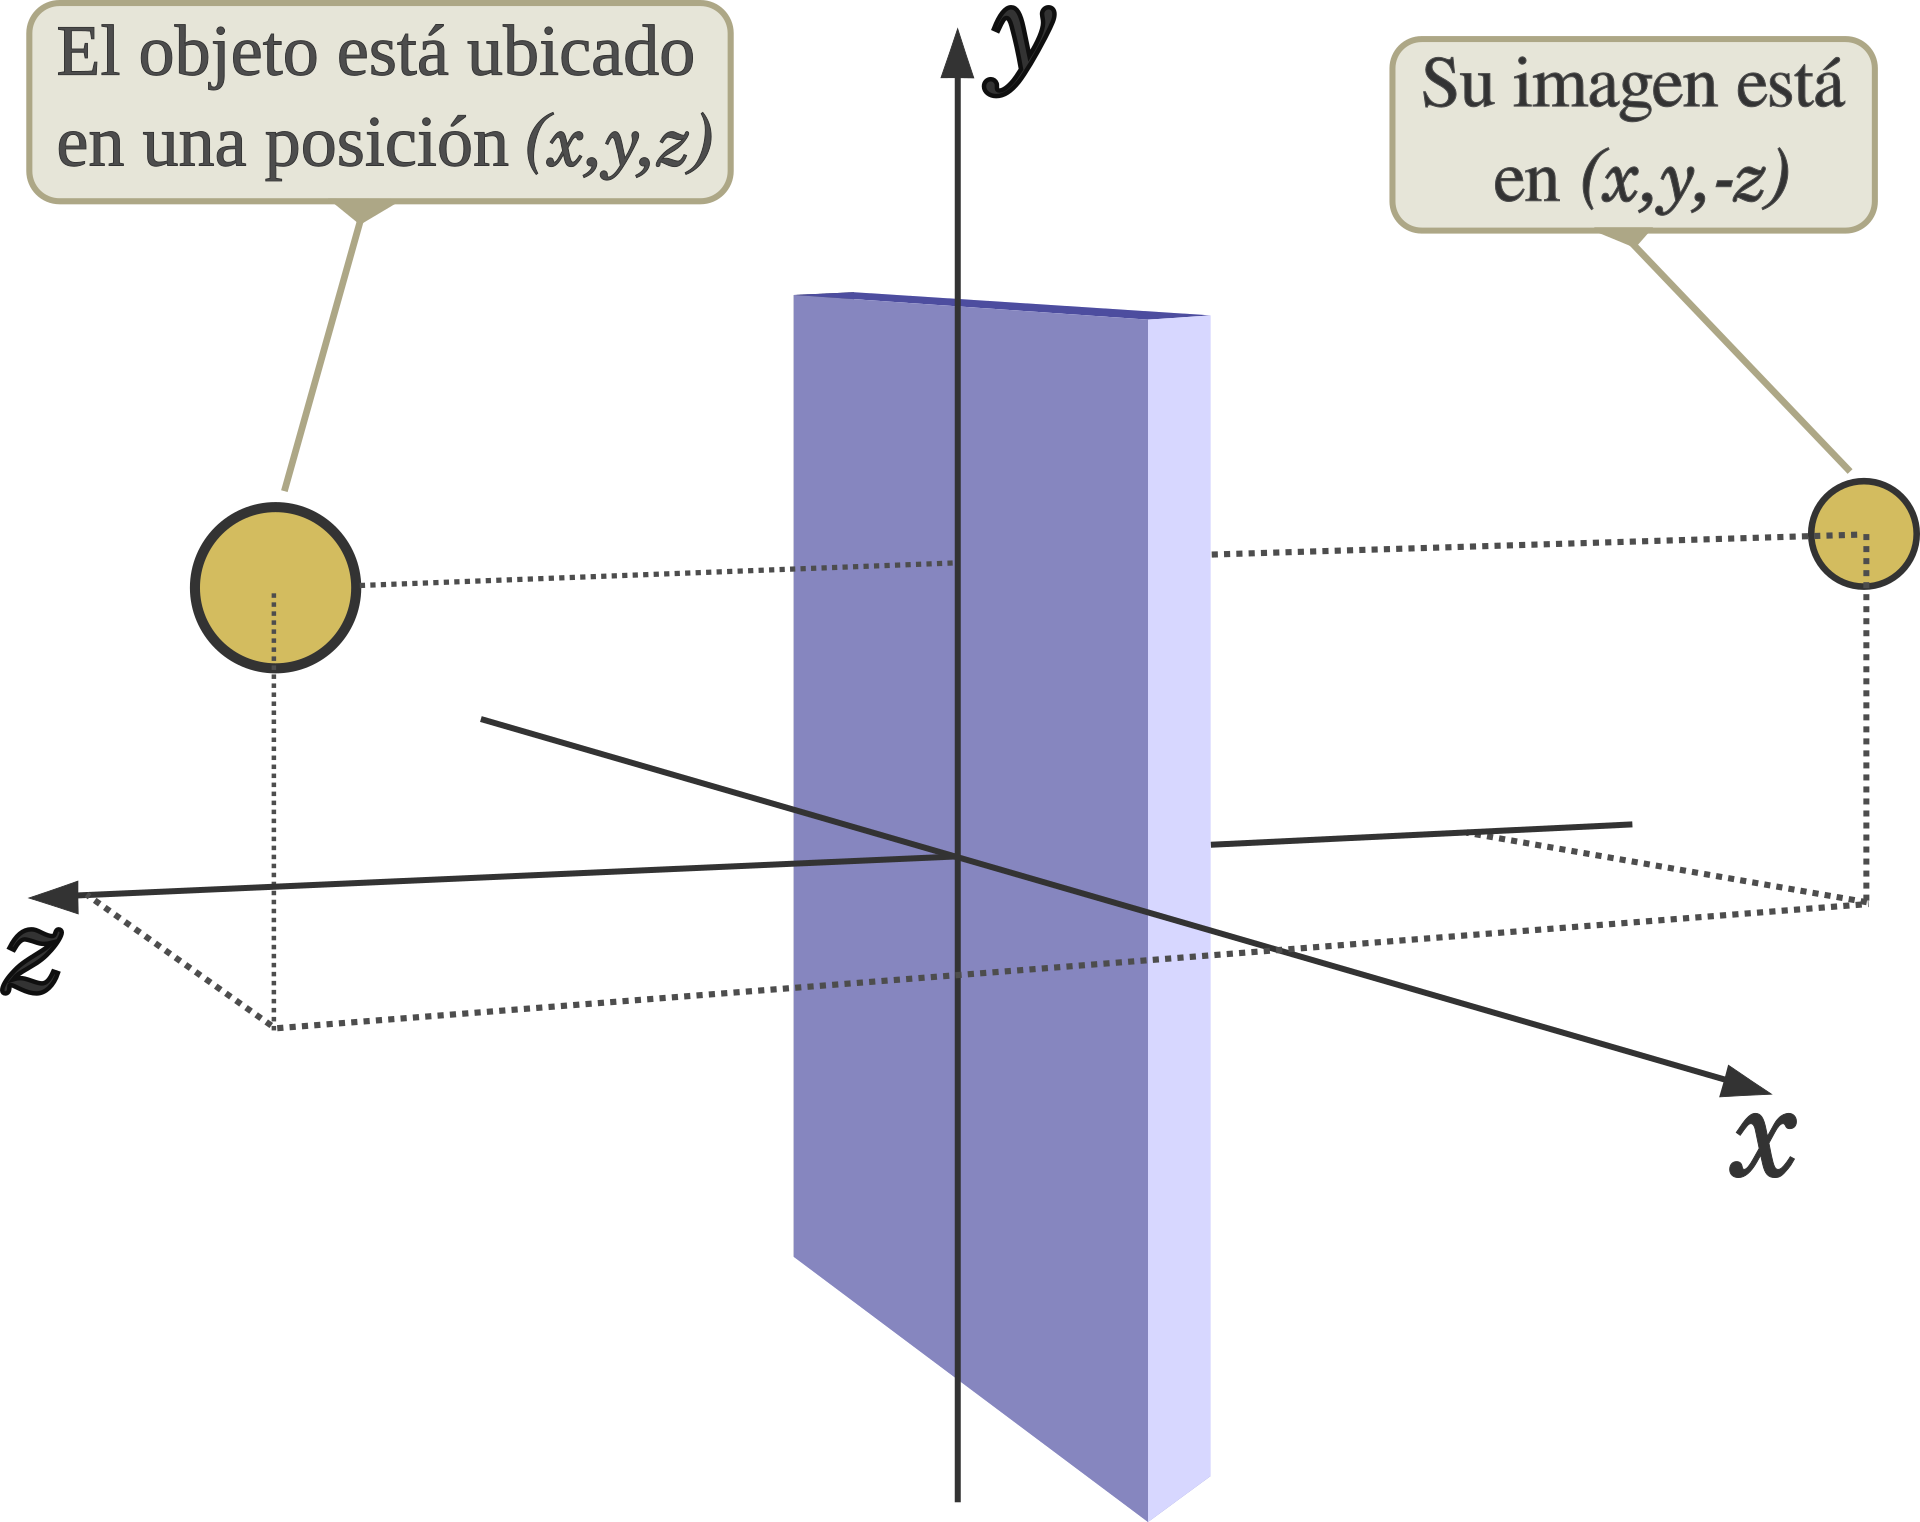
\includegraphics[width=\linewidth]{mirror_inversion.png}
  \caption{Inversión aparente de un espejo plano.}
  \label{fig:mirror_inversion}
\end{wrapfigure}
Matemáticamente, si representamos tu posición como un vector en el espacio tridimensional, por ejemplo \((x,y,z)\), el espejo refleja tu imagen como \((x,y,-z)\). Esto significa que solo se invierte el componente \(z\), que representa la profundidad (la distancia hacia el espejo).

¿Entonces por qué parece que se invierte la derecha y la izquierda? La confusión surge de la simetría especular y de cómo interpretamos las imágenes reflejadas. Si tú levantas tu mano derecha, la imagen parece levantar la mano izquierda solo porque está frente a ti, y tú la interpretas como una persona girada 180° sobre su eje vertical. En otras palabras, tu cerebro intenta interpretar la imagen como si fuera otra persona que se ha dado vuelta para mirarte, lo cual implicaría una inversión izquierda-derecha. Pero el espejo no realiza esa rotación: tú haces esa interpretación mental.

Un ejemplo claro: si sostienes un cartel con letras normales (no al revés) frente a un espejo, verás las letras invertidas horizontalmente. Esto no ocurre porque el espejo invierta la izquierda y la derecha, sino porque tú has girado el cartel hacia el espejo; si lo haces transparente y lo colocas de espaldas, la imagen coincidirá perfectamente.

\subsubsection{Imágenes formadas por espejos esféricos}

Ahora se estudiarán las imágenes formadas por espejos curvos. Aunque son posibles varias curvaturas, la investigación se restringirá a espejos esféricos. 

Un espejo esférico es aquel que tiene la forma de una sección de una esfera.

\paragraph{Espejo cóncavo}

Si tomamos la sección interna de una esfera, obtenemos un \textbf{espejo cóncavo}. Este tipo de espejos tienen su superficie curva hacia el objeto.
\begin{figure}[ht]
  \centering
  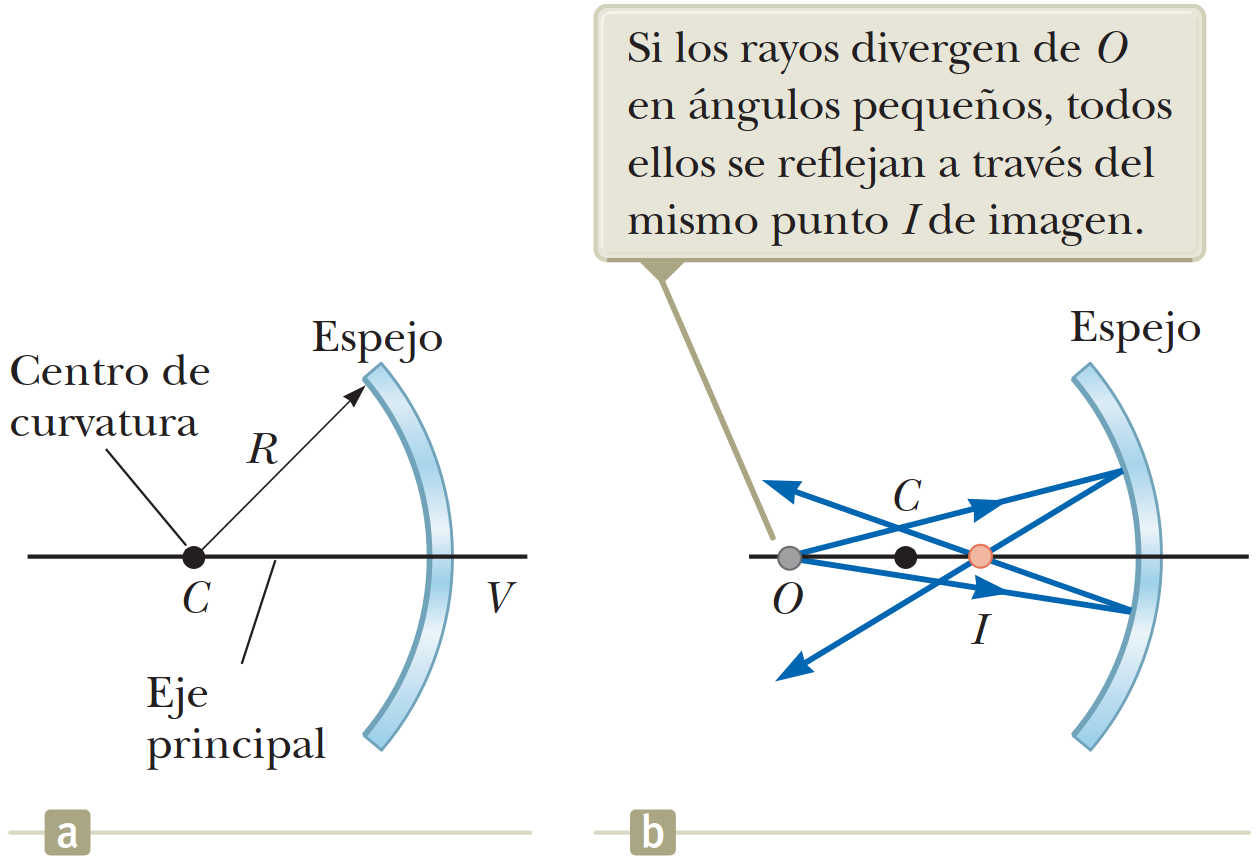
\includegraphics[width=0.55\textwidth]{mirror_concave.png}
  \caption{Elementos de un espejo cóncavo.}
  \label{fig:mirror_concave}
\end{figure}

La figura \ref{fig:mirror_concave}a muestra que el espejo tiene un radio de curvatura \(R\), y su centro de curvatura es el punto \(C\). El punto \(V\) es el centro de la sección esférica, y una línea a través de \(C\) y \(V\) se llama \textbf{eje principal} del espejo.

Ahora considere la figura \ref{fig:mirror_concave}b, que muestra un objeto ubicado en el punto \(O\), donde \(O\) es cualquier punto sobre el eje principal a la izquierda de \(C\). También se muestran dos rayos divergentes que salen del objeto, estos se reflejan en el espejo y convergen en el punto \(I\). Esta es la imagen del objeto \(O\). Luego los rayos continúan su trayecto divergente. Como resultado, la imagen \(I\) es \textbf{real}.

Solo vamos a considerar aquellos rayos que se reflejan en el espejo y convergen en el punto \(I\) del eje principal. A estos rayos se les llama \textbf{rayos paraxiales}. Existen rayos que no son paraxiales (convergen lejos del eje principal) y producen una imagen borrosa. A este efecto se le conoce como \textit{aberración esférica}.

Si se conoce la distancia \(p\) y el radio de curvatura \(R\), se puede calcular la distancia \(q\) de la imagen con la siguiente ecuación:
\begin{equation}
    \boxed{\frac{1}{p} + \frac{1}{q} = \frac{2}{R}}
    \label{eq:mirror_concave}
\end{equation}
Para comprender de dónde sale la ecuación \ref{eq:mirror_concave}, veamos la figura \ref{fig:mirror_concave_2}.

\begin{figure}[ht]
  \centering
  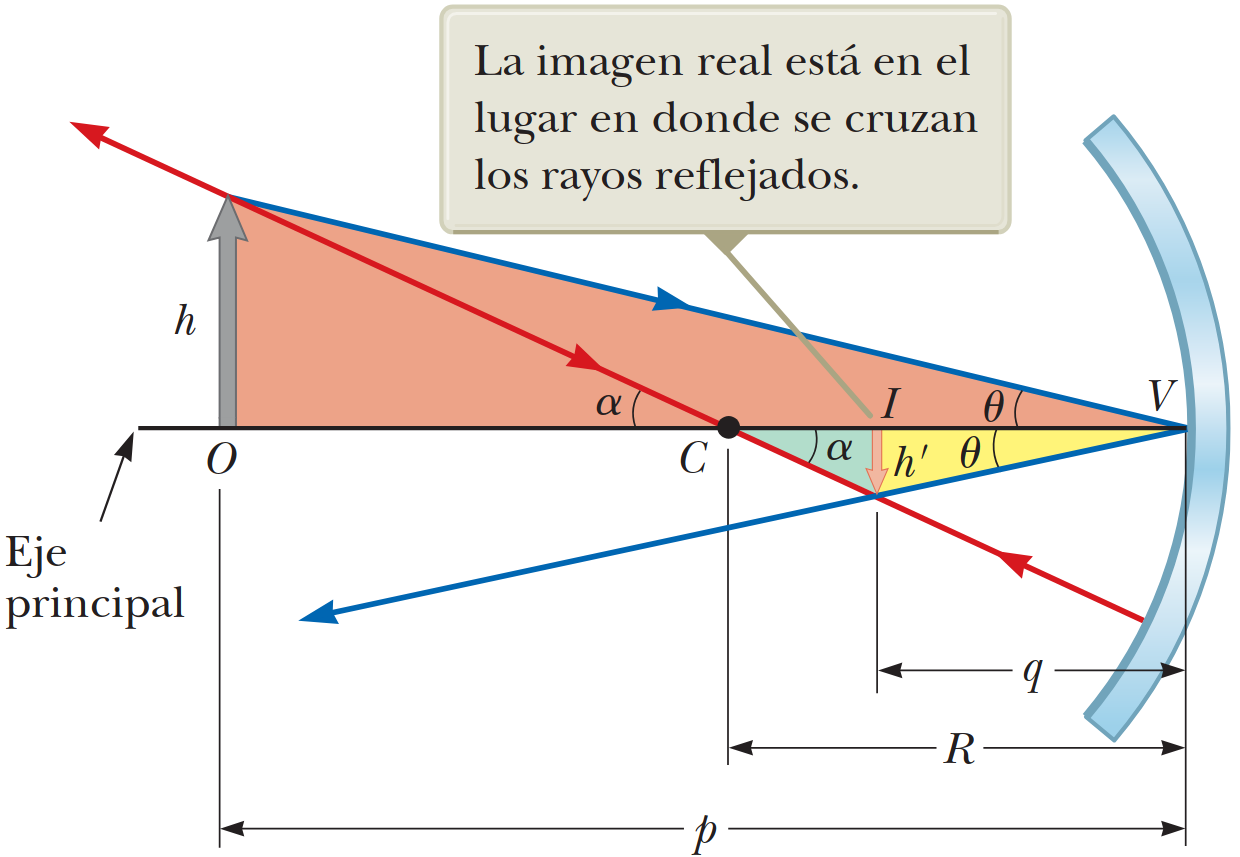
\includegraphics[width=0.6\textwidth]{mirror_concave_analysis.png}
  \caption{Imagen formada por un espejo esférico cóncavo cuando el objeto \(O\) yace fuera del centro de curvatura \(C\).}
  \label{fig:mirror_concave_2}
\end{figure}
En esta figura se ha puesto un objeto con forma de flecha (flecha gris) delante de un espejo cóncavo (espejo celeste). Este espejo proyecta una imagen real, amplificada y verticalmente invertida (flecha roja).

\begin{tcolorbox}[mydanger]
  Amplificación \textbf{no} necesariamente significa aumento.
\end{tcolorbox}

Como muestra la figura \ref{fig:mirror_concave_2}, dos rayos salen de la punta del una flecha. El rayo rojo pasa a través del centro de curvatura, e incide sobre el espejo perpendicular a la superficie, reflejándose de regreso sobre sí mismo.

El rayo azul incide en el espejo en su centro (punto \(V\)) y se refleja como se muestra. La imagen de la punta de la flecha se localiza en el punto donde se cruzan ambos rayos. Del triángulo rectángulo grande de color rojo puede ver que \(\tan(\theta) = h/p\), y del triangulo rectángulo amarillo se ve que \(\tan(\theta) = -h'/q\).\footnote{El signo negativo se debe a que la imagen es invertida y \(h'\) es negativo}

Operando sobre las expresiones trigonométricas:
\[
  \tan(\theta) = \frac{h}{p} = \frac{-h'}{q} \implies \frac{h'}{h} = -\frac{q}{p}
\]

Por lo tanto, de la ecuación \ref{eq:aumento_lateral} (aumento lateral) encontramos que el aumento de la imagen es:
\begin{equation}
  M = \frac{h'}{h} = -\frac{q}{p}
  \label{eq:aumento_lateral_concave}
\end{equation}

Si vemos el triangulo verde de la figura, tenemos que:
\[
  \tan(\alpha) = \frac{-h'}{R-q} \quad \text{y} \quad \tan(\alpha) = \frac{h}{p-R}
\]
Donde al sustituir en el aumento lateral resulta la ecuación \ref{eq:mirror_concave} que se denomina ecuación de espejo.

\begin{wrapfigure}{r}{0.33\textwidth}
  \centering
  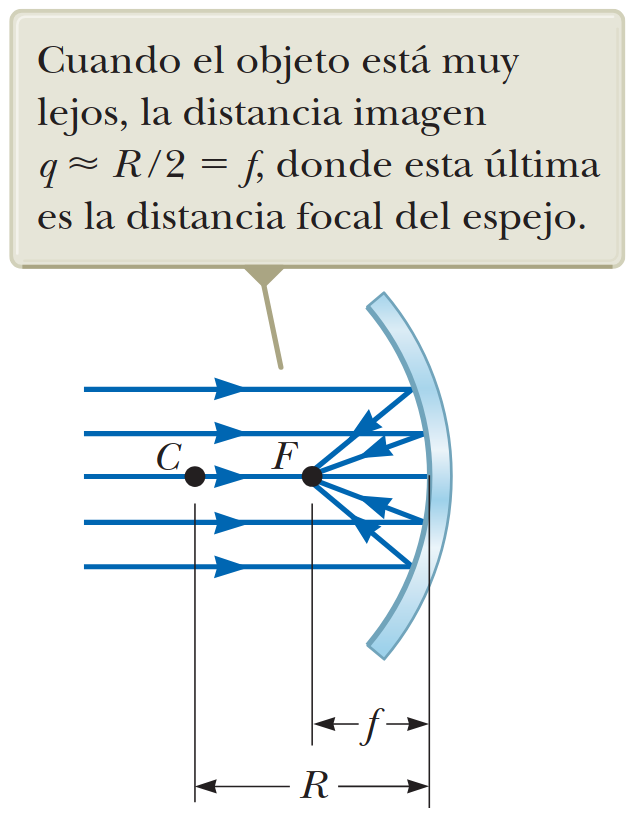
\includegraphics[width=\linewidth]{focal_distance.png}
  \caption{Foco de un espejo cóncavo.}
  \label{fig:focal_distance}
\end{wrapfigure}
El \textbf{foco} del espejo se puede determinar suponiendo que el objeto está muy alejado. En este caso la distancia \(p \to \infty\), y por lo tanto \(1/p \to 0\). 

En este caso especial, donde el objeto está infinitamente alejado, la imagen coincide con el foco. Por lo general, el foco no es el punto en el cual los rayos luminosos se enfocan para formar una imagen. El foco está determinado sólo por la curvatura del espejo, no depende de la posición del objeto. Por lo común, la imagen se forma en un punto distinto del foco de un espejo (o una lente). La \textit{única} excepción es cuando el objeto está infinitamente alejado, en este caso la imagen se forma en el foco.

Entonces, en el caso de la figura \ref{fig:focal_distance}, donde los rayos inciden de forma paralela, se puede suponer que la fuente está muy lejos, y el foco y la imagen coinciden. 
\begin{equation}
  \frac{1}{q} = \frac{2}{R} \implies f = \frac{R}{2}
  \label{eq:focal_distance}
\end{equation}
Al combinar las ecuaciones \ref{eq:mirror_concave} y \ref{eq:focal_distance}, obtenemos la \textbf{ecuación de espejo}:
\begin{equation}
  \frac{1}{p} + \frac{1}{q} = \frac{1}{f}
\end{equation}

\paragraph{Espejo convexo}

Si tomamos la sección interna de una esfera, obtenemos un \textbf{espejo convexo} también llamado espejo \textbf{divergente}, ya que los rayos de cualquier punto a un objeto divergen después de reflejarse. Este tipo de espejos tienen el pandeo hacia el objeto.

La imagen producida por un espejo convexo siempre es virtual, derecha y disminuida. Se dice que es disminuida cuando el aumento lateral es menor que 1, es decir, \(M < 1\).

No se deducirá ecuaciones para los espejos esféricos convexos, porque puede utilizar las ecuaciones \ref{eq:aumento_lateral_concave}, \ref{eq:mirror_concave} y \ref{eq:focal_distance} tanto para espejos cóncavos como para espejos convexos, siempre y cuando siga una regla.

\begin{figure}[ht]
  \centering
  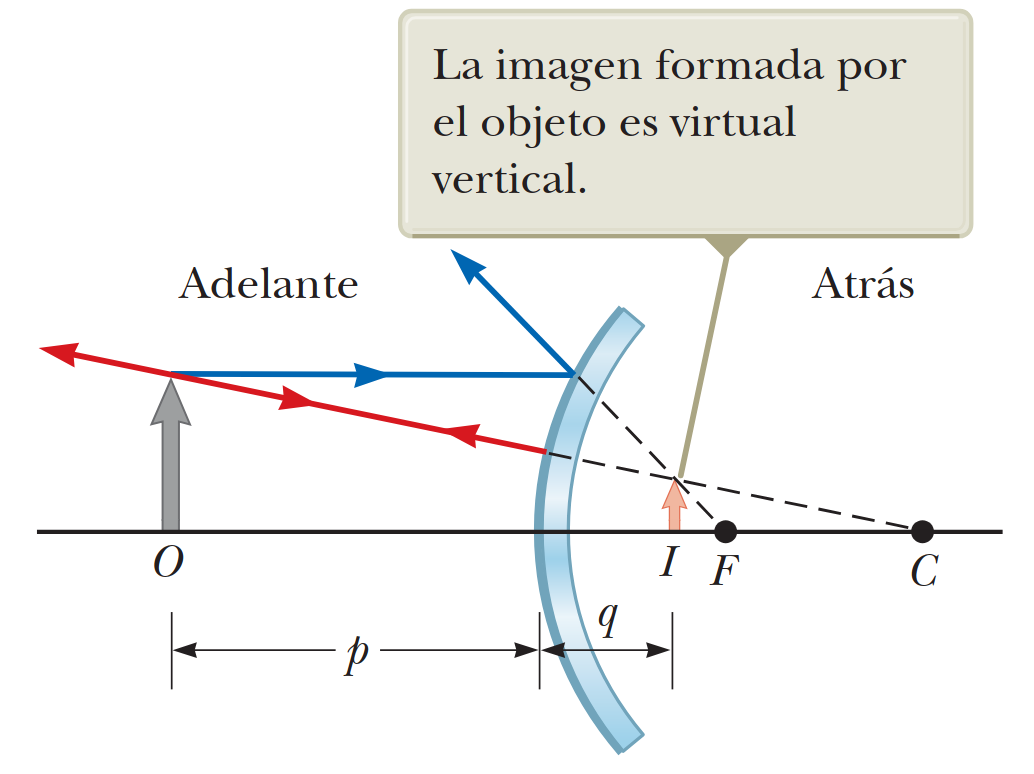
\includegraphics[width=0.55\textwidth]{convex_mirror.png}
  \caption{Elementos de un espejo convexo.}
  \label{fig:convex_mirror}
\end{figure}
Teniendo en cuenta la figura \ref{fig:convex_mirror}, el procedimiento es el siguiente:
\begin{enumerate}
  \item Identifique la región en la cual los rayos luminosos se mueven hacia el espejo como \textit{cara frontal} y el otro lado como \textit{cara trasera} (es decir la parte frontal que recibe los rayos y trasera del espejo que no recibe los rayos).
  \item Identifique la localización del objeto \(p\) teniendo en cuenta:
    \begin{itemize}
      \item el objeto está delante del espejo: \textit{objeto real} (positivo)
      \item el objeto está detrás del espejo: \textit{objeto virtual} (negativo)
    \end{itemize}
  \item  Localización de la imagen \(q\):
    \begin{itemize}
      \item la imagen está delante del espejo: \textit{imagen real} (positiva)
      \item la imagen está detrás del espejo: \textit{imagen virtual} (negativa)
    \end{itemize}
  \item Altura de la imagen \(h'\):
    \begin{itemize}
      \item la imagen es invertida: \(h' < 0\) (negativa)
      \item la imagen no es invertida: \(h' > 0\) (positiva)
    \end{itemize}
  \item Distancia focal \(f\) y radio \(R\):
    \begin{itemize}
      \item Es positiva cunado el espejo es cóncavo
      \item Es negativa cuando el espejo es convexo
    \end{itemize}
  \item Aumento lateral \(M\):
    \begin{itemize}
      \item la imagen es aumentada: \(M > 1\)
      \item la imagen es disminuida: \(M < 1\)
      \item la imagen es del mismo tamaño: \(M = 1\)
    \end{itemize}
\end{enumerate}

\subsubsection{Diagrama de rayos para los espejos}

El diagrama de rayos para los espejos es un diagrama que muestra la trayectoria de los rayos que salen de un objeto y se reflejan en un espejo. Es muy útil para verificar los cálculos realizados y entender la naturaleza de la imagen formada.

\noindent Para dibujar el diagrama de rayo es necesario conocer:
\begin{itemize}
  \item la posición del objeto \(p\)
  \item la localización del foco \(f\)
  \item el centro de curvatura del espejo \(C\)
\end{itemize}

\noindent A continuación se presentan ejemplos para los diagramas de rayos para los espejos cóncavos y convexos.

\subparagraph{Para espejos cóncavos}

Se tienen dos posibilidades:
\begin{enumerate}
  \item El objeto está ubicado detrás del foco y la imagen será real, invertida y aumentada.
  \item El objeto está ubicado entre el foco y el centro de curvatura y la imagen será virtual, derecha y disminuida.
\end{enumerate}

\begin{figure}[ht]
  \centering
  \begin{subfigure}[b]{0.51\textwidth}
      \centering
      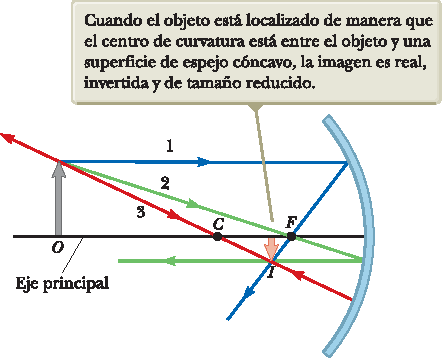
\includegraphics[width=\textwidth]{mirror_diagram_1.pdf}
      \caption{Diagrama de rayos para un espejo cuando el objeto está ubicado detrás del foco.}
      \label{fig:mirror_diagram_1}
  \end{subfigure}
  \hfill
  \begin{subfigure}[b]{0.45\textwidth}
      \centering
      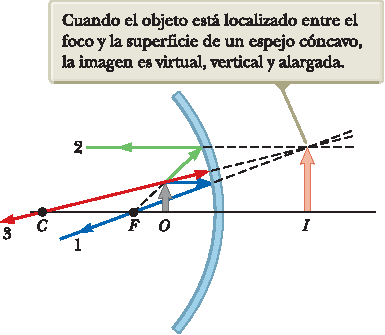
\includegraphics[width=\textwidth]{mirror_diagram_2.pdf}
      \caption{Diagrama de rayos para un espejo cuando el objeto está delante del foco.}
      \label{fig:mirror_diagram_2}
  \end{subfigure}
  \caption{Diagrama de rayos para espejos cóncavos}
  \label{fig:mirror_diagram}
\end{figure}

\noindent La estrategia es la siguiente: una vez se conocen los datos del problema, dibuje tres rayos principales para localizar la imagen. Estos son:

\begin{enumerate}
  \item Un rayo paralelo al eje principal, y el reflejo que pasa por el foco.
  \item El rayo que pasa por el foco \(f\), y el reflejo que es paralelo al eje principal.
  \item Un rayo que pasa por el centro de curvatura \(C\), y se refleja sobre sí mismo.
\end{enumerate}

\subparagraph{Para espejos convexos}

Se tiene una sola posibilidad: El objeto está ubicado entre el foco y el centro de curvatura y la imagen será virtual, derecha y disminuida.

\begin{figure}[ht]
  \centering
  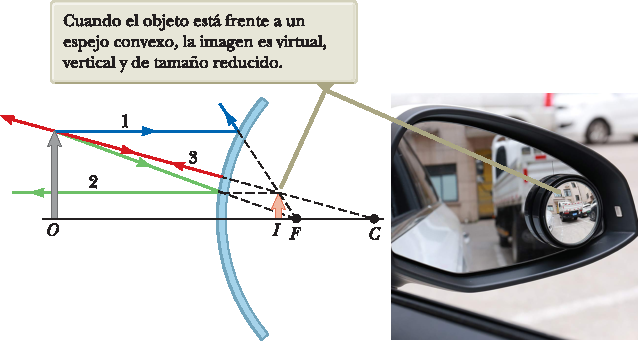
\includegraphics[width=0.6\textwidth]{mirror_diagram_3.pdf}
  \caption{Diagrama de rayos para un espejo convexo.}
  \label{fig:mirror_diagram_3}
\end{figure}

\subsubsection{Estrategia para resolver problemas de espejos}

\begin{tcolorbox}[interesting_data, title=Recuerda]
  Es muy importante que recuerdes que el objeto no ``emite'' rayos, la luz proviene de alguna fuente, y rebota en el objeto. Luego los rayos se reflejan en el espejo y forman la imagen.
  Los rayos que salen del objeto no son dos o tres, sino que son infinitos. Puedes dibujar tantos rayos como quieras. En este resumen se han dibujado los rayos más convenientes para localizar la imagen de forma rápida, pero podrías dibujar otros rayos para verificar los cálculos.
\end{tcolorbox}

\begin{wrapfigure}{r}{0.4\textwidth}
  \centering
  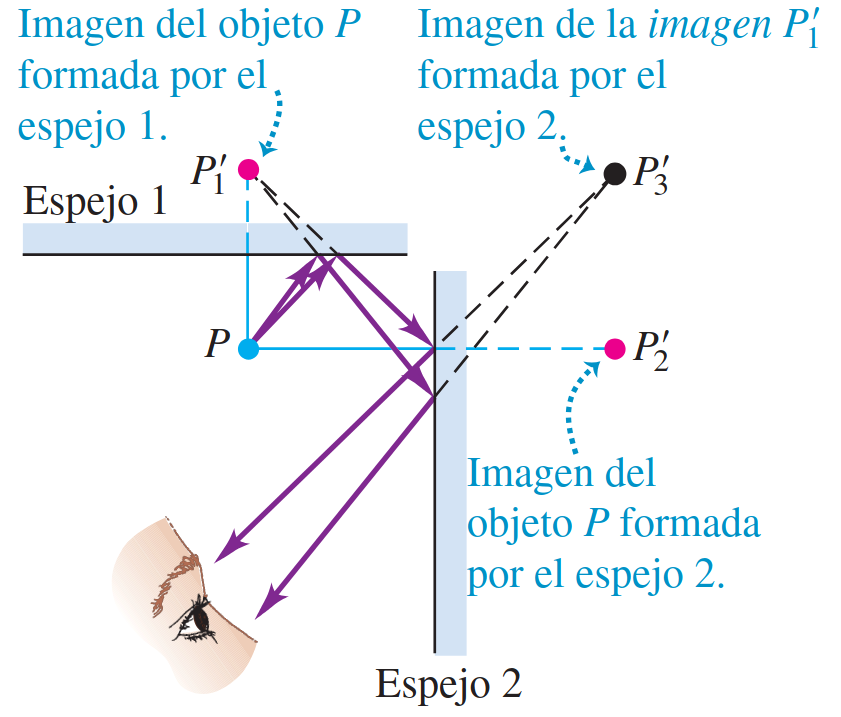
\includegraphics[width=\linewidth]{mirror_excercise.png}
  \caption{Dos espejos ubicados a 90 grados entre sí.}
  \label{fig:mirror_excercise}
\end{wrapfigure}
Un ejercicio común es el que se muestra en la figura \ref{fig:mirror_excercise}. Para resolver este ejercicio y descubrir por qué hay una tercer imagen, es necesario aplicar la recomendación del cuadro de arriba. 

Recordando entonces que los rayos que salen del objeto no son dos o tres, sino que son infinitos, es posible dibujar tantos rayos como quieras para encontrar todas las imágenes posibles.

Tal vez piense ¿Cómo se supone que dibuje infinitos rayos? No es necesario dibujar infinitos rayos, solo es necesario dibujar algunos como para entender el comportamiento de los rayos y cómo se forman las imágenes.

Veamos como sería para este ejemplo. Tenemos una partícula ubicada en el punto \(P\). Sabemos que, en cada espejo producirá una imagen, entonces tendremos la imagen \(P_1'\) para el espejo \(E_1\) y \(P_2'\) para el espejo \(E_2\).

Ahora, si continuamos trazando rayos, vemos que algunos rayos que rebotan en el espejo \(E_1\), luego rebotan en el espejo \(E_2\). Esto significa que parte del espejo \(E_1\) se refleja en el espejo \(E_2\).

Ahora, prestemos atención a este efecto: como el observador no está ubicado sobre la línea que une a la partícula \(P\) con la intersección entre los espejos, verá el reflejo del espejo \(E_1\) en el espejo \(E_2\). Esto significa que verá la imagen \(P_1'\) reflejada en el espejo \(E_2\), formando la imagen \(P_3'\).

La imagen \(P_3'\) es una imagen de la imagen \(P_1'\), es decir, es una imagen virtual, derecha y disminuida.